\section{Introduzione e requisiti}

\subsection{Descrizione del sistema}

SmartParking è un parcheggio automatico. Ci sono due sbarre, una in ingresso e una in
uscita, dei sensori che si accorgono quando arriva un'auto e un totem che legge che tipo
di utente è. I posti sono di due tipi: standard e riservati ai disabili. Nel modello ne
ho messo uno solo per tipo, altrimenti il model checker dopo esplode.
\\ \\
Gli utenti sono tre:

\begin{itemize}
\item \textbf{STD}: l'utente standard, è l'unico che paga;
\item \textbf{DISABILE}: ha il permesso, non paga e ha la precedenza sui posti riservati;
\item \textbf{ABBONATO}: ha l'abbonamento mensile e non paga.
\end{itemize}

Quando arriva un'auto il sistema la rileva, guarda che utente è e controlla se c'è un
posto adatto. Se c'è alza la sbarra, se non c'è nega l'accesso.
\\
Il caso un po' più interessante è quello del disabile. Lui i posti riservati li prende
per primo, ma se sono finiti il sistema non lo respinge: gli dà un posto standard, se ce
n'è uno libero. Questo è il \emph{fallback}. Solo se sono finiti anche i posti standard
viene negato l'accesso anche a lui.
\\
In uscita paga solo l'utente STD, gli altri due escono e basta.

\subsection{Requisiti funzionali}

\begin{longtable}{@{}p{1.3cm}p{9.5cm}p{2cm}@{}}
\toprule
\textbf{ID} & \textbf{Descrizione} & \textbf{Priorità} \\
\midrule
\endhead
RF1  & Rilevare l'arrivo di un veicolo in ingresso (\texttt{sens\_in}) e passare da IDLE a CHK\_IN. & Alta \\
RF2  & Identificare il tipo di utente (STD, DISABILE, ABBONATO) e passare allo stato VER. & Alta \\
RF3  & Per STD/ABBONATO, assegnare un posto standard se \texttt{posti\_std > 0} e aprire la sbarra (INGR). & Alta \\
RF4  & Per DISABILE, assegnare in via prioritaria un posto disabile se \texttt{posti\_dis > 0}. & Alta \\
RF5  & Se per un DISABILE i posti disabili sono esauriti, tentare il fallback su posto standard. & Alta \\
RF6  & Se nessun posto è disponibile (inclusi i fallback), negare l'accesso (NEG). & Alta \\
RF7  & Da NEG, tornare in IDLE solo dopo che il veicolo si è allontanato (\texttt{auto\_via}). & Media \\
RF8  & Al transito in ingresso, decrementare il contatore del posto assegnato e tornare in IDLE. & Alta \\
RF9  & Rilevare l'arrivo di un veicolo in uscita (\texttt{sens\_out}) e passare a CHK\_OUT. & Alta \\
RF10 & In uscita, per STD richiedere il pagamento (TARIF) prima della sbarra. & Alta \\
RF11 & In uscita, per DISABILE/ABBONATO saltare il pagamento e andare direttamente a USC. & Alta \\
RF12 & Restare in TARIF finché il pagamento non è confermato. & Alta \\
RF13 & Al transito in uscita, incrementare il contatore, azzerare la memoria del posto e tornare in IDLE. & Alta \\
RF14 & Mantenere in memoria il tipo di posto occupato dall'ingresso fino all'uscita. & Media \\
\bottomrule
\end{longtable}

\subsection{Requisiti non funzionali}

\begin{longtable}{@{}p{1.3cm}p{10.2cm}@{}}
\toprule
\textbf{ID} & \textbf{Descrizione} \\
\midrule
\endhead
RNF1 & \textbf{Sicurezza dei contatori}: \texttt{posti\_std} e \texttt{posti\_dis} non devono mai essere negativi né superare la capacità iniziale, in ogni stato raggiungibile. \\
RNF2 & \textbf{Determinismo}: a parità di stato e input monitorati, il sistema produce sempre lo stesso stato successivo. \\
RNF3 & \textbf{Assenza di stati bloccanti}: da ogni stato transitorio esiste sempre un cammino che riporta il sistema in IDLE. \\
\bottomrule
\end{longtable}

Tutti e tre sono stati verificati formalmente, e vale la pena dire con cosa. RNF1 è
esattamente il contenuto delle CTLSPEC da 1 a 6 sul modello e delle due invarianti di
classe JML su \texttt{Parcheggio}: la stessa proprietà dimostrata due volte, una sul
modello astratto e una sul codice.

RNF2 merita una precisazione, perché la regola di assegnazione usa un \texttt{choose},
che è un costrutto non deterministico. Il determinismo non viene meno: come spiegato in
Sezione~\ref{sec:modello}, l'insieme fra cui il \texttt{choose} sceglie contiene sempre
al massimo un elemento, quindi lo stato successivo resta univoco.

RNF3 corrisponde alla CTLSPEC~8, \texttt{ag(stato=TARIF implies ef(stato=IDLE))}, che
risulta vera. È importante che sia formulato con ``esiste un cammino'' e non ``su tutti i
cammini'': la versione forte è la CTLSPEC~10, con \texttt{af} al posto di \texttt{ef}, ed
è \emph{falsa}, perché un utente che non paga mai resta in TARIF per sempre. Il requisito
è scritto nella forma debole apposta.

\subsection{Tracciabilità}

Ogni requisito funzionale è verificato ad almeno due livelli, sul modello astratto e sul
codice. La tabella mette in fila chi controlla cosa.

\begin{longtable}{@{}p{1.3cm}p{5.2cm}p{6cm}@{}}
\toprule
\textbf{ID} & \textbf{Verifica sul modello} & \textbf{Verifica sul codice} \\
\midrule
\endhead
RF1--RF2 & \texttt{test\_abbonato}, \texttt{test\_disabile} & \texttt{SmartParkingFSMTest} (transizioni IDLE$\to$CHK\_IN$\to$VER) \\
RF3 & \texttt{test\_abbonato}, \texttt{test\_pieno} & \texttt{ParcheggioTest}, \texttt{McdcVerificaTest} (decisione 1) \\
RF4 & \texttt{test\_disabile} & \texttt{ParcheggioTest}, riga 3 della tabella pairwise \\
RF5 & \texttt{test\_disabile\_fallback} & \texttt{McdcVerificaTest} (decisione 2), riga 4 pairwise \\
RF6 & \texttt{test\_pieno\_totale}, CTLSPEC~9 & \texttt{DisplayMockTest}, riga 1 pairwise \\
RF7 & \texttt{test\_pieno} & \texttt{SmartParkingFSMTest} (self-loop di NEG) \\
RF8 & \texttt{test\_abbonato}, CTLSPEC~3 e~6 & \texttt{SmartParkingFSMTest}, \texttt{ScenarioAvallaTest} \\
RF9 & \texttt{test\_pagamento\_std} & \texttt{SmartParkingFSMTest} \\
RF10 & \texttt{test\_pagamento\_std}, CTLSPEC~7 & \texttt{SmartParkingFSMTest} \\
RF11 & \texttt{test\_abbonato}, \texttt{test\_disabile} & \texttt{SmartParkingFSMTest} \\
RF12 & \texttt{test\_pagamento\_std} & \texttt{SmartParkingFSMTest} (self-loop di TARIF) \\
RF13 & \texttt{test\_disabile}, CTLSPEC~4 e~5 & \texttt{ParcheggioTest} (\texttt{liberaPosto}) \\
RF14 & \texttt{test\_disabile} & \texttt{SmartParkingFSMTest} \\
\bottomrule
\caption{Tracciabilità dei requisiti funzionali verso scenari, proprietà temporali e test.}
\label{tab:tracciabilita}
\end{longtable}

\subsection{Macchina a stati}

Qui sotto ci sono gli 8 stati del modello e le transizioni che li collegano. Il giro
sopra è quello di ingresso, quello sotto l'uscita, e da IDLE si parte sempre.

\begin{figure}[H]
    \centering
    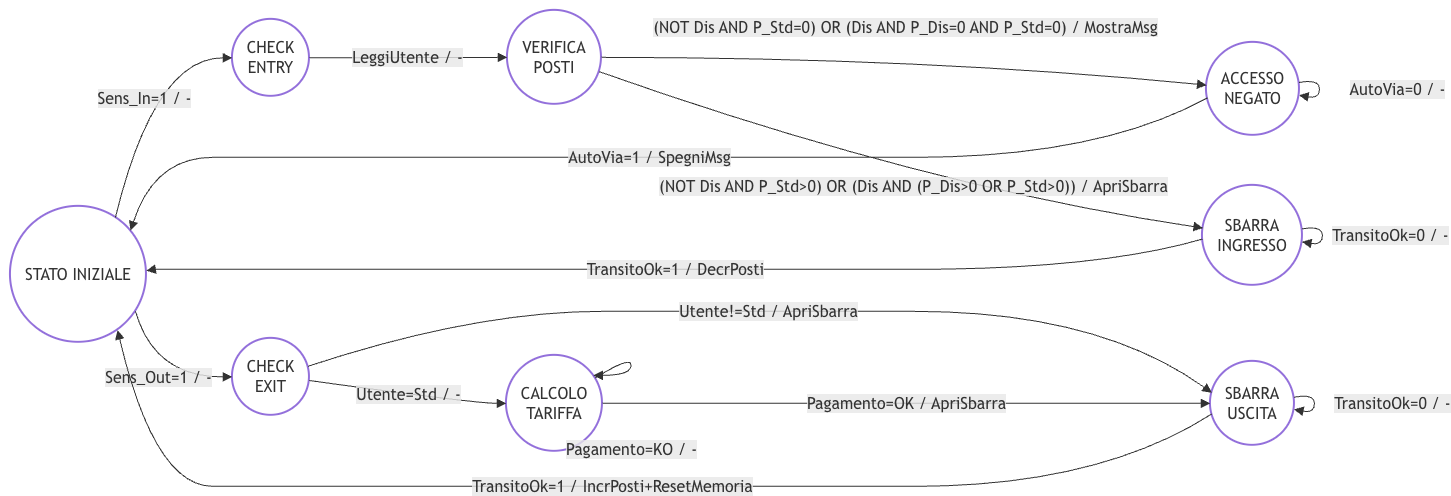
\includegraphics[width=1\linewidth]{images/ASM.drawio.png}
    \caption{Macchina a stati di SmartParking: gli 8 stati e le transizioni, con il ciclo
    di ingresso (CHK\_IN, VER, INGR oppure NEG) e quello di uscita (CHK\_OUT, TARIF, USC).}
    \label{fig:fsm}
\end{figure}



\newpage